

\documentclass[crop,tikz]{standalone}% 'crop' is the default for v1.0, before it was 'preview'
\usepackage{pgfplots}
\pgfplotsset{compat=newest}
\usetikzlibrary{calc}
\usetikzlibrary{shapes.geometric}
\usetikzlibrary{decorations.pathreplacing,calligraphy}
\usetikzlibrary{shapes,arrows,chains}

\begin{document}
\begin{tikzpicture}

\node[] at (0,0) {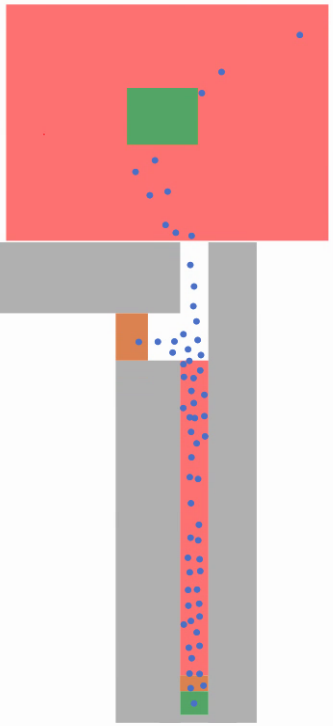
\includegraphics[height=8.0cm]{unguided_130.png}};
\node[] at (3.5,0) {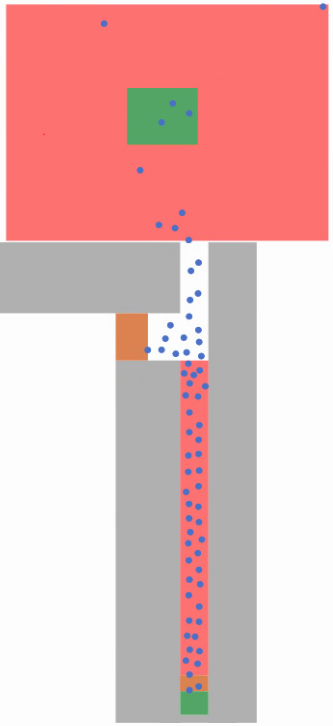
\includegraphics[height=8.0cm]{unguided_140.png}};
\node[] at (7,0) {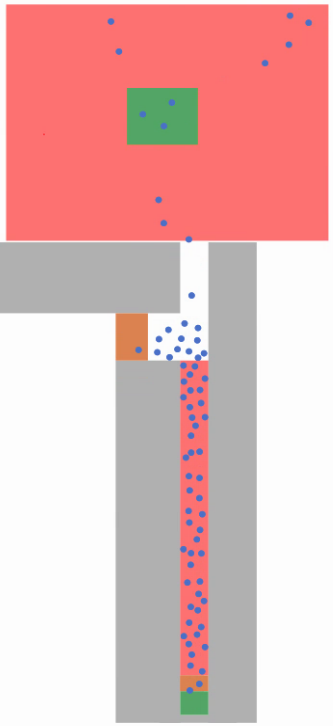
\includegraphics[height=8.0cm]{unguided_150.png}};
\node[] at (10.5,0) {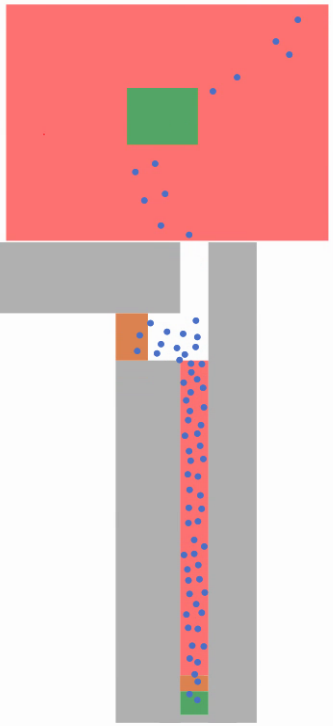
\includegraphics[height=8.0cm]{unguided_160.png}};
\node[] at (5.6,4.7) {\textbf{Without guidance}};
\node[] at (0,4.3) {Sim. time: 130s};
\node[] at (3.5,4.3) {140s};
\node[] at (7,4.3) {150s};
\node[] at (10.5,4.3) {160s};


\node[] at (0,-9.0) {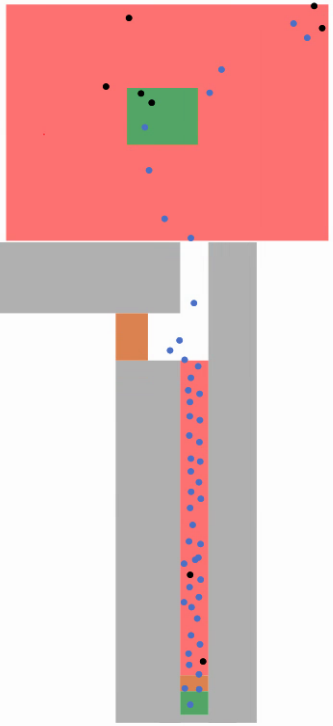
\includegraphics[height=8.0cm]{guided_130.png}};
\node[] at (3.5,-9.0) {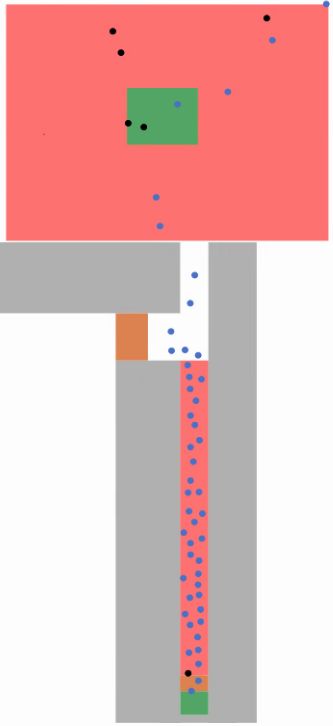
\includegraphics[height=8.0cm]{guided_140.png}};
\node[] at (7,-9.0) {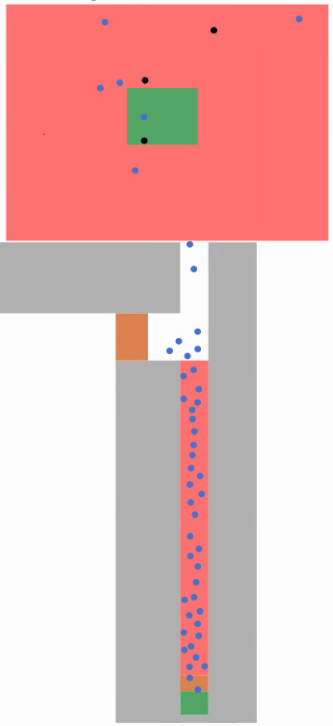
\includegraphics[height=8.0cm]{guided_150.png}};
\node[] at (10.5,-9.0) {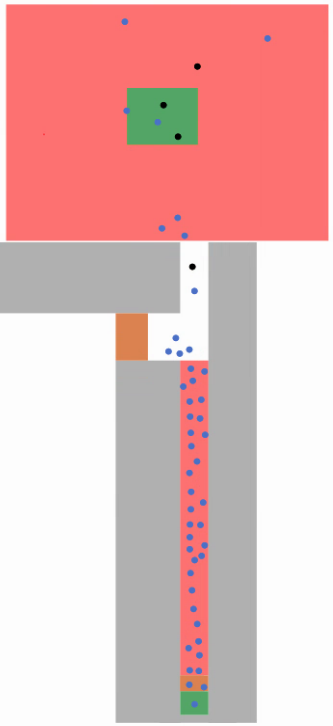
\includegraphics[height=8.0cm]{guided_160.png}};

\node[] at (6,-4.3) {\textbf{With guidance (long route recommended)}};
\node[] at (0,-4.7) {Sim. time: 130s};
\node[] at (3.5,-4.7) {140s};
\node[] at (7,-4.7) {150s};
\node[] at (10.5,-4.7) {160s};

%5\draw[->] (-0.85,-5.5) -- (-0.85,-5.1);
%\draw[->] (-0.6,-5.4) -- (-0.6,-5.0);

%\draw[->] (2.7,-5.7) -- (2.7,-5.4);
%\draw[->] (3.0,-5.7) -- (3.0,-5.4);

%\draw[->] (4.2,-5.4) -- (4.5,-5.1);
%\draw[->] (4.4,-5.5) -- (4.6,-5.2);

%\draw[->] (6.15,-5.0) -- (6.15,-4.7);


%\draw[->] (10.9,-5.9) -- (11.1,-5.6);
\draw[->] (10.9,-5.7) -- (11.1,-5.5);

\end{tikzpicture}
\end{document}